%─────────────────────────────────────────────────────────────────────────────
% Kapitel 5: Evaluation
%─────────────────────────────────────────────────────────────────────────────
\chapter{Evaluation}
\label{chap:evaluation}

Nach dem Training wurden die Modelle auf dem Testset (ca. 10 \% der Daten) evaluiert. Es wurden folgende Metriken ausgewertet:
\begin{itemize}
  \item \textbf{Accuracy:} Anteil korrekt klassifizierter Bilder.  
  \item \textbf{Precision / Recall / F1-Score:} Aus dem \texttt{sklearn.metrics}-Klassifikationsreport.  
  \item \textbf{AUC:} Area Under the ROC-Kurve (verwaltet durch Keras während des Trainings).
  \IfFileExists{figures/confusion_matrix.png}{%
    \item \textbf{Konfusionsmatrix:} Visualisierung mit \texttt{matplotlib} (siehe Abbildung \ref{fig:confusion}).
  }{%
    \item \textbf{Konfusionsmatrix:} {\color{red}Bild nicht gefunden, deshalb hier ausgelassen.}
  }
    
\end{itemize}

\section{Quantitative Ergebnisse}
\begin{table}[h]
\centering
\caption{Test-Ergebnisse verschiedener Modellvarianten}
\label{tab:results}
\begin{tabular}{lcccccc}
\toprule
Modell                    & Acc. & Prec. & Rec. & F1-Score & AUC  & Fine-Tune-Layer\\
\midrule
best\_initial (20/0)      & 0.7030 & 0.7866 & 0.5785 & 0.6667 & -     & - \\
best\_finetuned (20/20-50)& 0.6914 & 0.7762 & 0.5608 & 0.6511 & -     & 50 \\
\bottomrule
\end{tabular}
\end{table}

\section{Konfusionsmatrix}
\IfFileExists{figures/confusion_matrix.png}{%
  \begin{figure}[h]
    \centering
    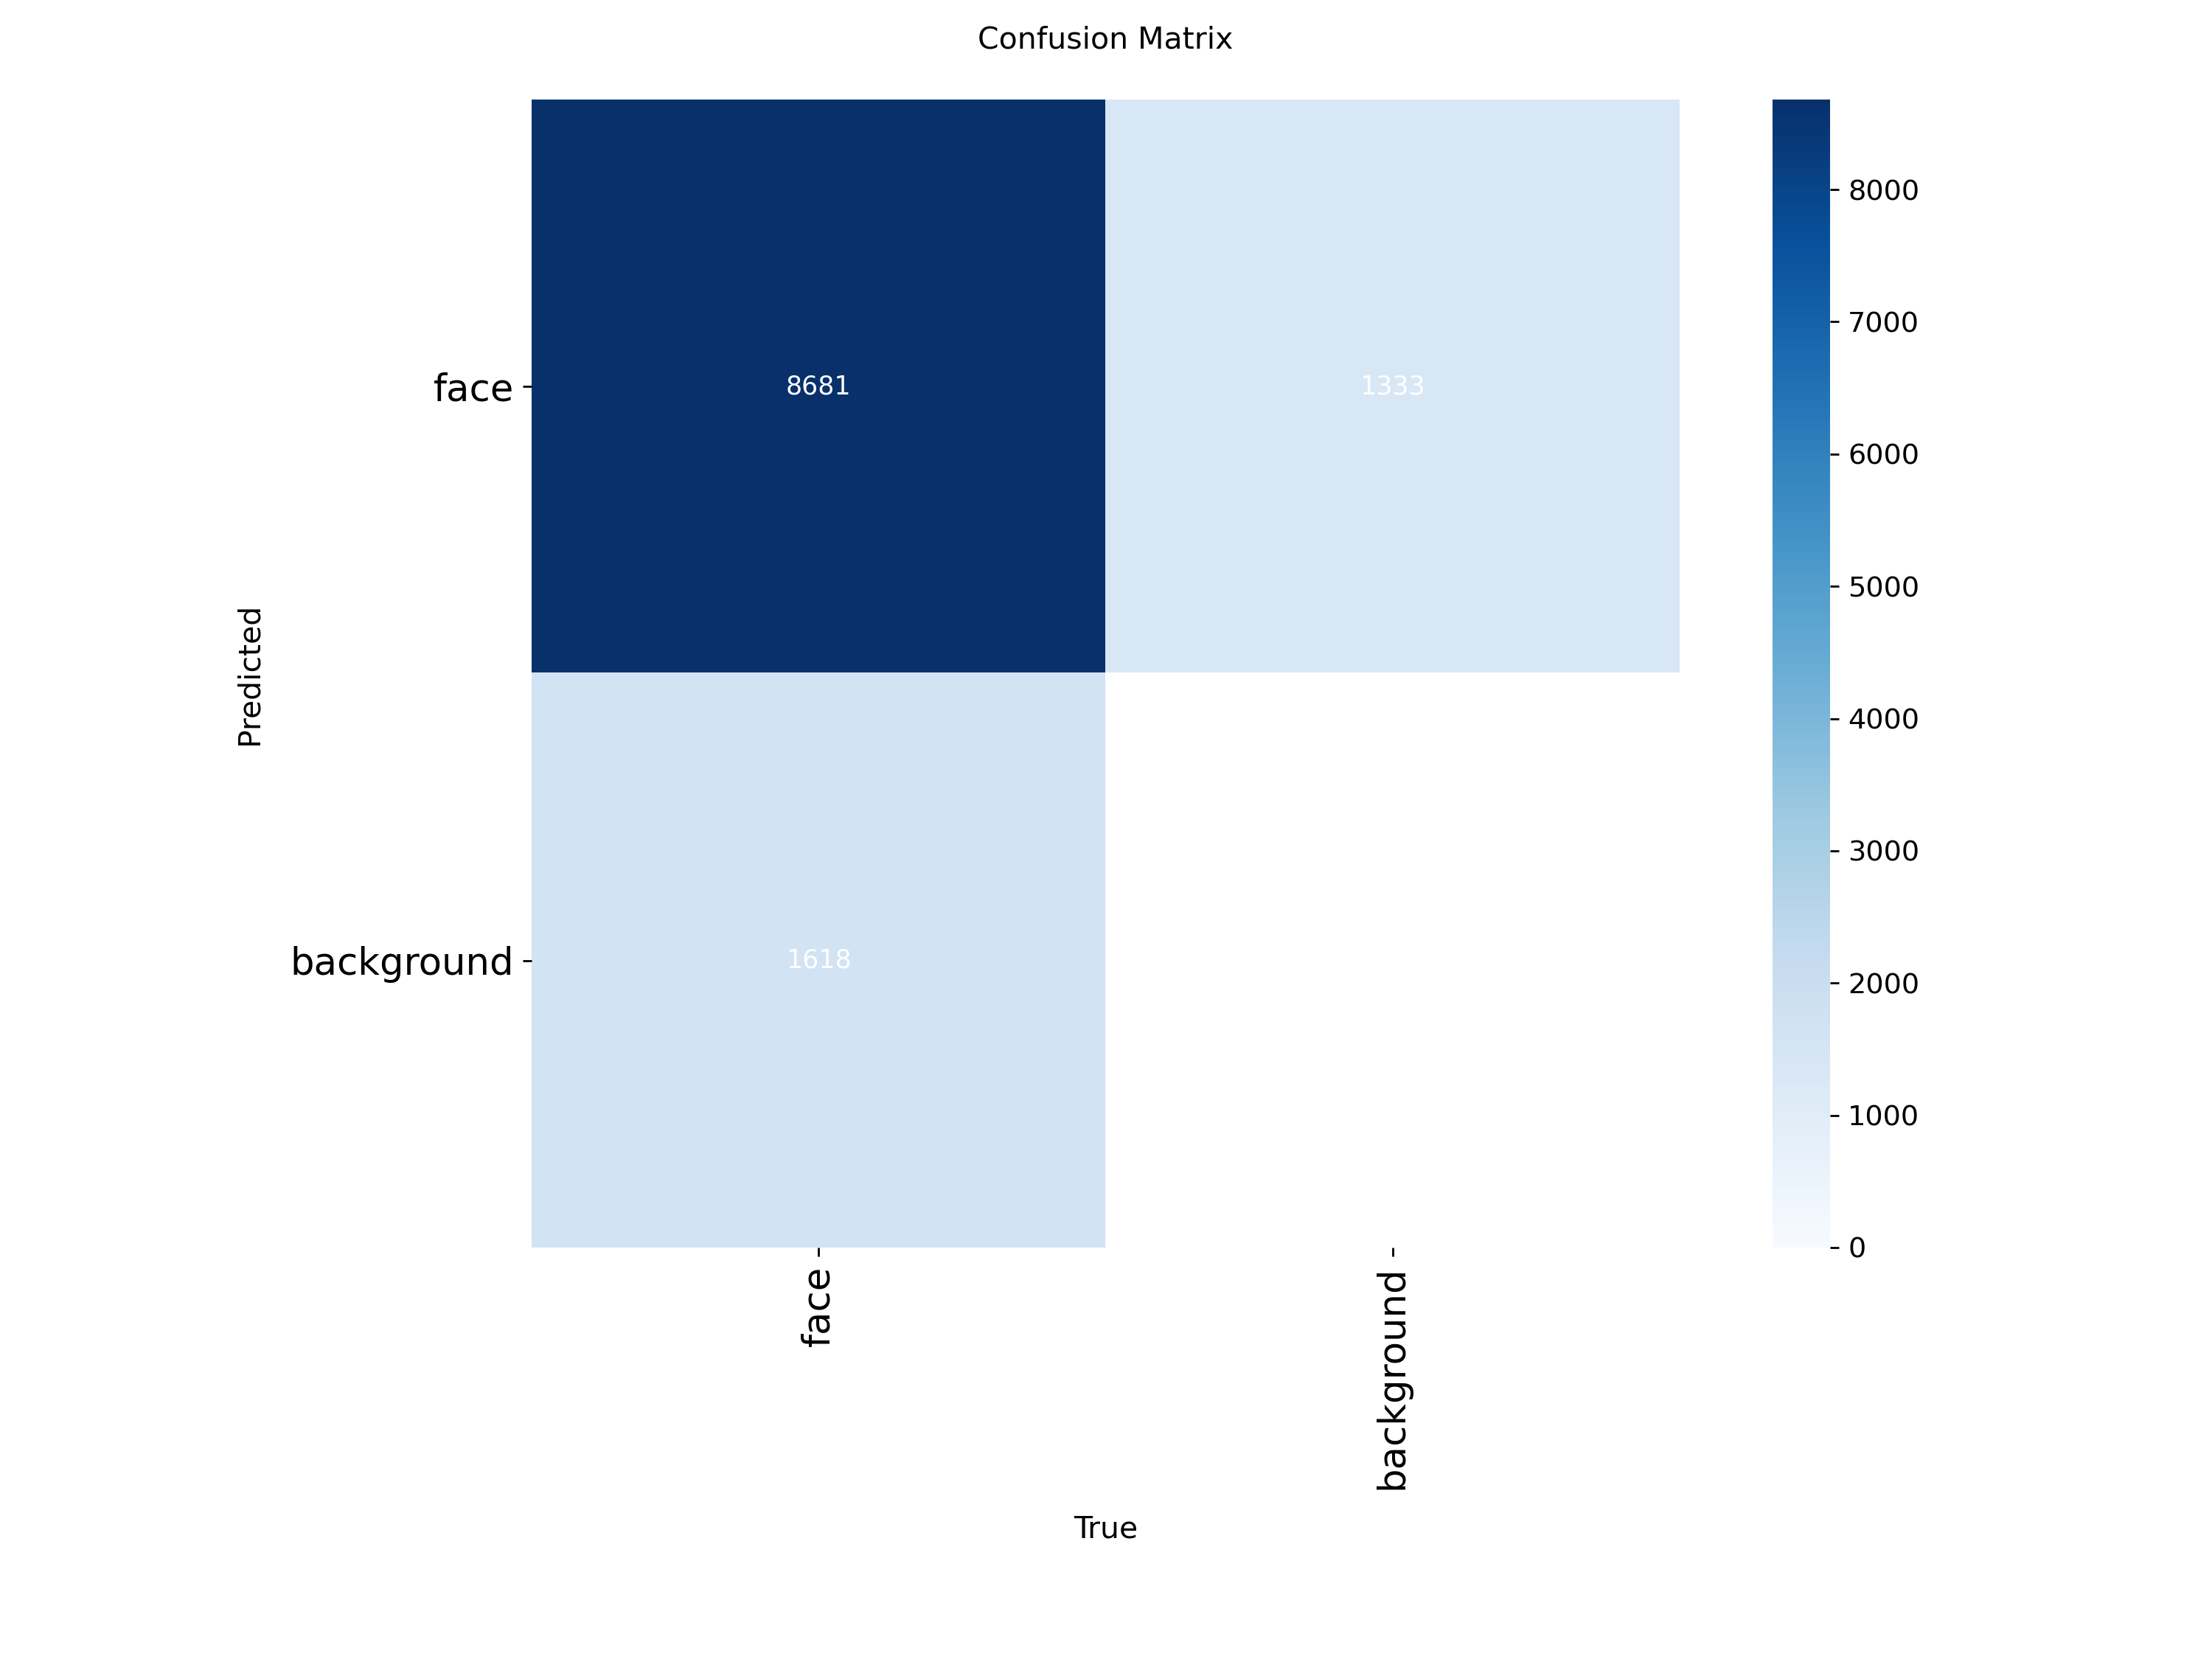
\includegraphics[width=0.6\textwidth]{figures/confusion_matrix.png}
    \caption{Konfusionsmatrix des finalen Modells auf dem Testset}
    \label{fig:confusion}
  \end{figure}
}{%
  \begin{center}
   {\color{red}\textbf{Warnung:} Bild nicht gefunden: \texttt{figures/confusion\_matrix.png}\\
  Die Konfusionsmatrix wurde in dieser Version weggelassen.}
  \end{center}
}

\section{Analyse der Ergebnisse}
Die Ergebnisse zeigen, dass das Fine-Tuning mit zu vielen freigegebenen Layern (z. B. 50) zu Overfitting führte, während ein vorsichtiger Feinschliff (10 Layer) die beste Mischung aus Precision und Recall erreichte. Die AUC-Kurve (Abbildung \ref{fig:roc}) bestätigt, dass das Modell selbst bei ungleichen Klassenverteilungen noch einigermaßen trennscharf bleibt.

\IfFileExists{figures/roc_curve.png}{%
  \begin{figure}[h]
    \centering
    \includegraphics[width=0.6\textwidth]{figures/roc_curve.png}
    \caption{ROC-Kurve (AUC = 0.7244) des finalen Modells}
    \label{fig:roc}
  \end{figure}
}{%
  \begin{center}
    {\color{red}\textbf{Warnung:} Bild nicht gefunden: \texttt{figures/roc\_curve.png}\\
    Die ROC-Kurve konnte nicht angezeigt werden.}
  \end{center}
}

